\chapter{基因与 DNA}\label{ch:g9:genes-and-dna}

\omterm{def:g9:chromosomes:chromosomes}{染色体}携带着决定因子——但一条丝线
还不是一段文字。沿\omterm{def:g9:chromosomes:chromosomes}{染色体}，一个决定因子\emph{究竟是}什么？
而这条丝线由什么构成，竟能让一个宽仅千分之几毫米的
\omterm{def:g6:cell-unit-of-life:parts}{细胞核}容纳
整个人的全部指令
（见\cref{exo:g9:heredity-and-traits:12}）？答案是两个名字，
它们是现代生物学中最著名的：\omterm{def:g9:genes-and-dna:gene}{基因}，
以及 \omterm{def:g9:genes-and-dna:dna}{DNA}。

\section{基因：被定位的决定因子}

\begin{definition}[基因与等位基因]\label{def:g9:genes-and-dna:gene}
\emph{基因}\index{基因}是被精确定位的一个决定因子：
即\emph{\omterm{def:g9:chromosomes:chromosomes}{染色体}片段}，携带着构建某一\omterm{def:g9:heredity-and-traits:traits}{性状}部分所需的指令——
例如一个基因负责血型机制，另一些负责眼色色素，
成千上万，沿 46 条\omterm{def:g9:chromosomes:chromosomes}{染色体}排列，
各居其固定位置。
一个基因可以有几种版本——
\emph{等位基因}\index{等位基因}：血型基因的 A、B
与 O 三个版本，眼色基因的棕色与蓝色。
位置相同，拼写不同。
\end{definition}

\begin{proposition}[两个拷贝，以及“表现”的含义]\label{prop:g9:genes-and-dna:twocopies}
\omterm{def:g9:chromosomes:chromosomes}{染色体}成对出现
（见\cref{prop:g9:chromosomes:counts}）——因此每个\omterm{def:g9:genes-and-dna:gene}{基因}
都有\emph{两份拷贝}，每条同源\omterm{def:g9:chromosomes:chromosomes}{染色体}各一份，分别来自
父母。两份拷贝可以是相同的\omterm{def:g9:genes-and-dna:gene}{等位基因}，也可以不同；
不同时，其中一个可能\emph{表达}，另一个
则沉默地携带——家族相册里的谜团，
便可归结为机制：
\begin{itemize}
  \item 携带而不表现
        （见\cref{ex:g9:heredity-and-traits:skip}）：
        沉默的\omterm{def:g9:genes-and-dna:gene}{等位基因}由另一条同源\omterm{def:g9:chromosomes:chromosomes}{染色体}携带；
  \item A 型与 B 型父母所生的 O 型子女
        （见\cref{pb:g9:heredity-and-traits:1}）：父母各自
        都沉默地携带一个 O，减数分裂时的减半把两个 O
        同时分给了子女；
  \item 棕眼父母所生的蓝眼子女：两个沉默的蓝
        \omterm{def:g9:genes-and-dna:gene}{等位基因}相遇——当父母各携带一个蓝时，
        几率为四分之一：减半时，每位父母各把蓝
        \omterm{def:g9:genes-and-dna:gene}{等位基因}传递给子女的几率为二分之一，两次
        传递相互独立。
\end{itemize}
\end{proposition}
\admitted

\begin{example}[血型的完整机制]\label{ex:g9:genes-and-dna:bloodgroups}
一个\omterm{def:g9:genes-and-dna:gene}{基因}，三种\omterm{def:g9:genes-and-dna:gene}{等位基因}，每人两份拷贝：A 与 A
或 O 表现为 A 型；B 与 B 或 O 表现为 B 型；A 与 B 表现为
AB 型（两者均表达——\omterm{def:g9:genes-and-dna:gene}{等位基因}并非总是
可以沉默）；O 与 O 表现为 O 型。献血登记中的
全部规律——包括每一个“意外”——
都是两份拷贝组合的算术。
\end{example}

\section{DNA：文字的书写载体}

\begin{definition}[DNA]\label{def:g9:genes-and-dna:dna}
从化学角度看，\omterm{def:g9:chromosomes:chromosomes}{染色体}是一条极长、卷曲的
\emph{DNA}\index{DNA}分子（连同包装蛋白质）：
双链结构——即那著名的扭曲梯子——其
梯级是四种化学字母的配对。\emph{沿链的字母
排列顺序即为信息}：一个
\omterm{def:g9:genes-and-dna:gene}{基因}就是这段序列的一段，正如句子是
书页的一段。四种字母，仅一个人体便有三十亿个，
足以写下构建整个人体的全部指令，
卷曲在每一个\omterm{def:g6:cell-unit-of-life:parts}{细胞核}之中。
\end{definition}

\begin{example}[亲手观察]\label{ex:g9:genes-and-dna:extraction}
可以在厨房里提取 \omterm{def:g9:genes-and-dna:dna}{DNA}：捣碎香蕉或洋葱，
加入盐水和少量洗洁精（膜被破坏——
\cref{def:g6:cell-unit-of-life:parts}中的包膜正是其作用对象），
过滤后，在其上轻覆一层冷酒精：
交界处便升起一团白色的
细丝，可用牙签卷绕。这些细丝便是 \omterm{def:g9:genes-and-dna:dna}{DNA}
——正是本章所讨论的真实分子，
切切实实以厘米计量的实物。
\end{example}

\begin{omfigure}
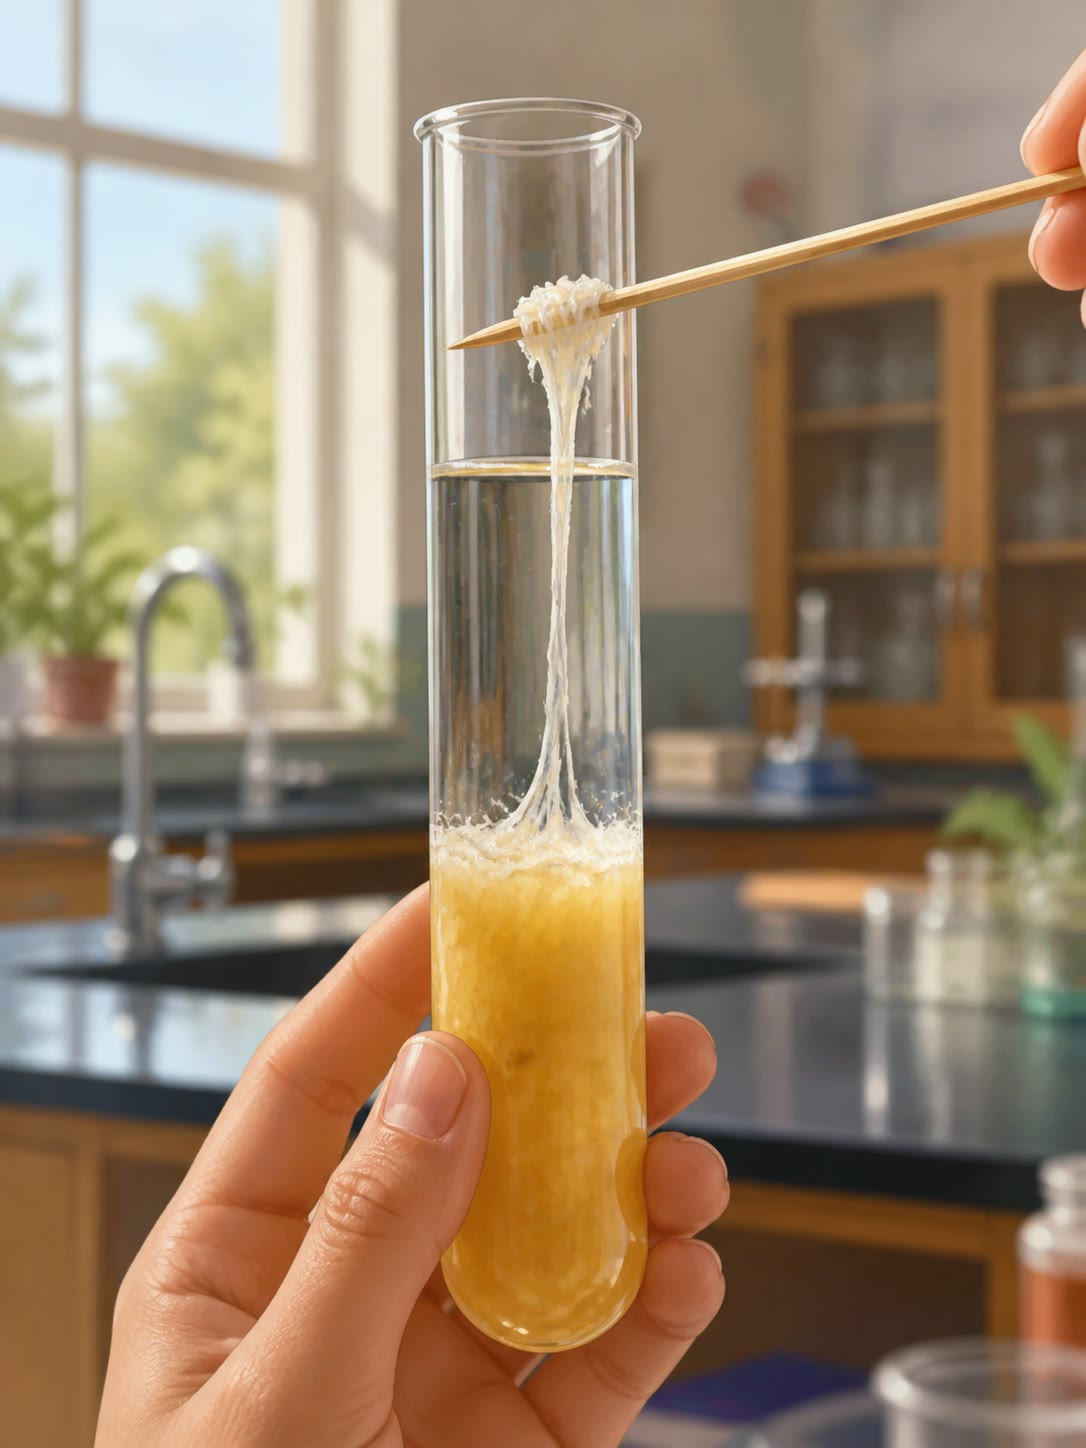
\includegraphics[width=0.42\linewidth]{images/book1/ai/g9-dna-extraction.jpg}

{\small 厨房提取的成果：\omterm{def:g9:heredity-and-traits:heredity}{遗传}的分子，
缠绕在牙签上。}
\end{omfigure}

\begin{proposition}[DNA 结构所能解释的问题]\label{prop:g9:genes-and-dna:explains}
双链并非装饰——每一种性质
都回答一个古老的问题：
\begin{itemize}
  \item \emph{复制}
        （\cref{prop:g5:first-look-at-cells:growth}所说的
        忠实分裂）：两条链的字母逐一互补，
        因此拉开后，
        各自都能重建其伙伴——一个梯子变成
        两个相同的梯子，分别进入每个子\omterm{def:g5:first-look-at-cells:cell}{细胞}；
  \item \emph{\omterm{def:g9:genes-and-dna:gene}{等位基因}}：\omterm{def:g9:genes-and-dna:gene}{基因}的各个版本，不过是序列中的
        微小拼写差异——
        位置相同，字母有所改变；
  \item \emph{突变}\index{突变}：复制
        近乎完美，但并非完美——偶尔一个字母被错抄，
        便产生了一个\emph{新}的\omterm{def:g9:genes-and-dna:gene}{等位基因}。多数中性，
        有时有害，偶尔有利：\omterm{prop:g9:genes-and-dna:explains}{突变}是新拼写的来源，
        归根结底，一切\omterm{def:g9:genes-and-dna:gene}{等位基因}都由此而来——
        这正是
        \cref{ch:g9:how-species-change}所需的原始素材；
  \item \emph{读取}：\omterm{def:g5:first-look-at-cells:cell}{细胞}利用\omterm{def:g9:genes-and-dna:gene}{基因}的方式，是读取其
        序列，并构建相应的工作分子——
        而每类\omterm{def:g5:first-look-at-cells:cell}{细胞}所读取的，是文库中自己的
        那一部分：
        \cref{exo:g9:chromosomes:12}中的谜题，
        如所承诺的那样得以解开。
\end{itemize}
\end{proposition}
\admitted

\begin{remark}[万物一码]\label{rem:g9:genes-and-dna:universal}
最深刻的事实留到最后：\emph{每一种}\omterm{def:g6:exploring-our-environment:components}{生物}
都用相同的 \omterm{def:g9:genes-and-dna:dna}{DNA} 字母书写其\omterm{def:g9:genes-and-dna:gene}{基因}，并以
同一套密码阅读它们——橡树、\omterm{ex:g6:producing-our-food:bread}{酵母}、鲸、
\cref{ch:g6:producing-our-food}中的\omterm{def:g6:producing-our-food:fermentation}{微生物}，以及你。这正是\omterm{prop:g5:first-look-at-cells:principle}{生命的统一性}
（\cref{prop:g5:first-look-at-cells:principle}）的根基，
也是\omterm{prop:g6:classification-kinship:kinship}{亲缘关系}树的
（\cref{rem:g6:classification-kinship:implies}）迄今最有力的证据：
共同的语言说明共同的起源。
这也正是\omterm{def:g9:genes-and-dna:gene}{基因}工程得以成立的原因——一个\omterm{def:g9:genes-and-dna:gene}{基因}
能在\omterm{def:g5:biodiversity:species}{物种}之间转移后仍可读取，如同一句被
复印到另一本书中的话。
\end{remark}

\begin{method}[三层次阅读]\label{met:g9:genes-and-dna:levels}
现在，任何\omterm{def:g9:heredity-and-traits:heredity}{遗传}问题都可以从三个层次来读——
练习在各层次间切换：
\begin{enumerate}
  \item \emph{家族层次}：谁表现、谁携带、谁
        传递（\cref{ch:g9:heredity-and-traits}）；
  \item \emph{\omterm{def:g9:chromosomes:chromosomes}{染色体}层次}：哪些\omterm{def:g9:chromosomes:chromosomes}{染色体}，经减半与
        复原，携带这一分配
        （\cref{ch:g9:chromosomes}）；
  \item \emph{分子层次}：哪个\omterm{def:g9:genes-and-dna:gene}{基因}、哪些\omterm{def:g9:genes-and-dna:gene}{等位基因}，
        何种拼写——若是新\omterm{def:g9:heredity-and-traits:traits}{性状}，则是何种
        \omterm{prop:g9:genes-and-dna:explains}{突变}。
\end{enumerate}
同一个故事，三种放大率；一个答案只有在
三个层次上都讲通时才算完整。
\end{method}

\section{练习}

\begin{exercise}[$\star$]\label{exo:g9:genes-and-dna:1}
结合血型的例子，给出\omterm{def:g9:genes-and-dna:gene}{基因}和\omterm{def:g9:genes-and-dna:gene}{等位基因}的定义。
\end{exercise}

\begin{exercise}[$\star$]\label{exo:g9:genes-and-dna:2}
为什么每个\omterm{def:g9:genes-and-dna:gene}{基因}都成对出现，它们位于
何处？
\end{exercise}

\begin{exercise}[$\star$]\label{exo:g9:genes-and-dna:3}
从物理上看，\omterm{def:g9:genes-and-dna:dna}{DNA} 的信息是什么？人类的“牌组”中有多少个字母，
共有几种？
\end{exercise}

\begin{exercise}[$\star$]\label{exo:g9:genes-and-dna:4}
双链结构如何使复制
得以忠实进行？
\end{exercise}

\begin{exercise}[$\star$]\label{exo:g9:genes-and-dna:5}
什么是\omterm{prop:g9:genes-and-dna:explains}{突变}？它可能具有的
三种性质分别是什么？
\end{exercise}

\begin{exercise}[$\star$]\label{exo:g9:genes-and-dna:6}
叙述\cref{rem:g9:genes-and-dna:universal}中的事实，以及
由其导出的两条推论。
\end{exercise}

\begin{exercise}[$\star\star$]\label{exo:g9:genes-and-dna:7}
从机制上解释褐眼父母所生蓝眼孩子的\omterm{def:g9:heredity-and-traits:heredity}{遗传}过程：
复制、分配，以及四分之一的概率。
\end{exercise}

\begin{exercise}[$\star\star$]\label{exo:g9:genes-and-dna:8}
完成\cref{ex:g9:genes-and-dna:bloodgroups}：列出
四个血型各自对应的\omterm{def:g9:genes-and-dna:gene}{等位基因}对。
\end{exercise}

\begin{exercise}[$\star\star$]\label{exo:g9:genes-and-dna:9}
用本章的术语解答\cref{exo:g9:chromosomes:12}：
\omterm{def:g8:nervous-communication:neuron}{神经元}读取了哪些\omterm{def:g1:the-five-senses:sense}{皮肤}\omterm{def:g5:first-look-at-cells:cell}{细胞}
所不读取的内容？
\end{exercise}

\begin{exercise}[$\star\star$]\label{exo:g9:genes-and-dna:10}
描述厨房里的提取过程，以及每种
厨房原料各自的作用。
\end{exercise}

\begin{exercise}[$\star\star$]\label{exo:g9:genes-and-dna:11}
依\cref{met:g9:genes-and-dna:levels}的三个层次，
分析\cref{pb:g9:heredity-and-traits:1}中的礼拜堂下巴。
\end{exercise}

\begin{exercise}[$\star\star\star$]\label{exo:g9:genes-and-dna:12}
“\omterm{prop:g9:genes-and-dna:explains}{突变}书写，洗牌发牌，表达展示。”
为每个动词指定其机制与所属章节——并指出
三者中哪一个真正产生\emph{新的}
拼写。
\end{exercise}

\section{问题：损坏的复印机}

\begin{problem}[{周末问题——追踪一个基因，
从拼写到家谱}]\label{pb:g9:genes-and-dna:1}
追踪一个（虚构但典型的）案例：一个色素\omterm{def:g9:genes-and-dna:gene}{基因}，
其有功能的\omterm{def:g9:genes-and-dna:gene}{等位基因} P 合成\omterm{def:g1:the-five-senses:sense}{皮肤}和毛发的色素；
很久以前，一次复制错误产生了损坏的\omterm{def:g9:genes-and-dna:gene}{等位基因} p——
拼写错误到无法读取，无法合成任何东西。携带 P
与 p 的个体外表正常；获得 p 与 p 的孩子不合成
任何色素——头发和\omterm{def:g1:the-five-senses:sense}{皮肤}非常白皙，对阳光脆弱的
眼睛（该情况存在于许多\omterm{def:g5:biodiversity:species}{物种}中）。

\medskip\noindent\textbf{第一部分——分子层次。}
\begin{enumerate}
  \item 指出 p 的起源，依据
        \cref{prop:g9:genes-and-dna:explains}，指出 p 的起源——
        一次性地，在某位祖先的
        生殖\omterm{def:g5:first-look-at-cells:cell}{细胞}系中物理上发生了什么？
  \item 为什么 P 与 p 的个体外表正常？哪个术语
        描述 p 的这种“搭乘”方式？
  \item 为什么 p 与 p 的个体会改变合成？缺少的是什么，
        它属于哪一章所讨论的哪一类
        机器（\cref{def:g9:genes-and-dna:gene}）？
  \item 该情况出现在许多\omterm{def:g5:biodiversity:species}{物种}中。依据
        \cref{rem:g9:genes-and-dna:universal}，它们的色素\omterm{def:g9:genes-and-dna:gene}{基因}拼写
        会有怎样的预测？
\end{enumerate}

\medskip\noindent\textbf{第二部分——\omterm{def:g9:chromosomes:chromosomes}{染色体}与
家族层次。}
\begin{enumerate}[resume]
  \item 两位携带者亲代（各含 P 与 p）：列出
        一个子代的四种等可能组合，以及
        pp \omterm{def:g9:genes-and-dna:gene}{基因}型个体的概率。
  \item 他们的 pp 女儿出生于两位
        外表正常的亲代。哪一个相册谜题
        （\cref{ex:g9:heredity-and-traits:skip}）刚刚
        完整地展现了其机制？
  \item 该女儿与 PP 型配偶所生的子女：
        他们都携带什么，又都不会表现
        出什么？
  \item 追踪一次传递中该\omterm{def:g9:genes-and-dna:gene}{等位基因}的“载体”：
        p 从祖母到孙辈的“搭乘”路径，
        逐条\omterm{def:g9:chromosomes:chromosomes}{染色体}、逐个\omterm{def:g8:sexual-reproduction:gametes}{配子}地追踪。
\end{enumerate}

\medskip\noindent\textbf{第三部分——三层次
论述。}
\begin{enumerate}[resume]
  \item 在
        \cref{met:g9:genes-and-dna:levels}中，按
        三个层次各写一句，描述该案例。
  \item 一位同学问，为何那个损坏的拼写
        早就未被简单地“修复掉”？请以携带者
        的正常外观作答：p 在哪里躲过了对其
        效应的任何评判？
  \item 防晒对女儿的重要性超过其携带者亲代。用一
        句话将\omterm{def:g9:heredity-and-traits:traits}{性状}、\omterm{def:g9:genes-and-dna:gene}{等位基因}对与\omterm{def:g6:exploring-our-environment:components}{环境}联系起来
        （沿用
        \cref{prop:g9:heredity-and-traits:sorting}
        的思路）。
  \item 以精确化的复印机图像作结：
        什么被复制，什么曾被错误地复制一次，
        以及为何该错误现在被忠实地复制。
\end{enumerate}
\end{problem}
